\documentclass[tikz,border=8pt]{standalone}
\usepackage{amsmath}
\usetikzlibrary{arrows.meta,positioning}
\begin{document}
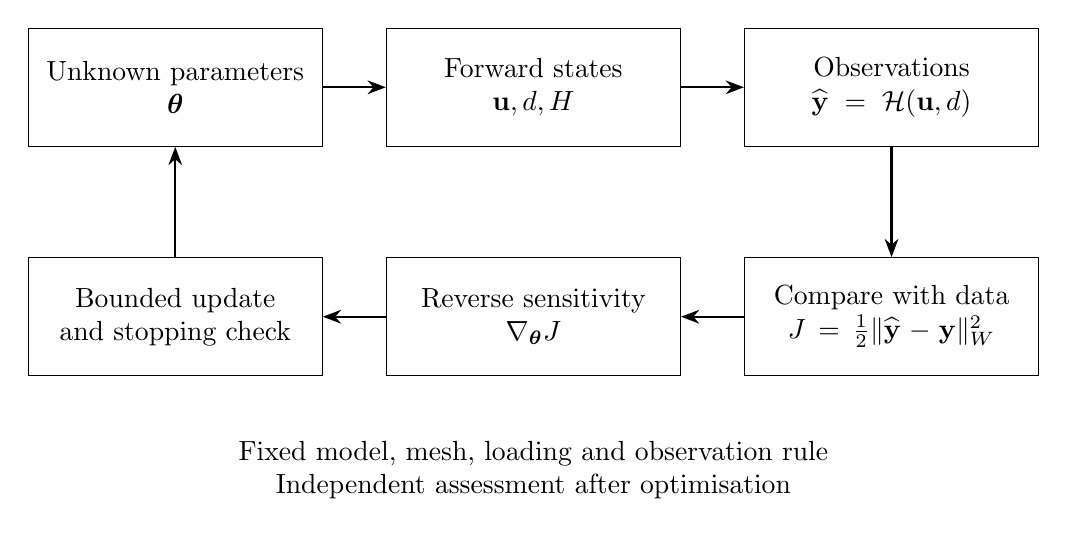
\begin{tikzpicture}[>=Stealth,font=\normalsize,
box/.style={draw,align=center,text width=35mm,minimum height=15mm},
arr/.style={->,line width=.8pt}]
\node[box] (p) {Unknown parameters\\$\boldsymbol\theta$};
\node[box,right=8mm of p] (f) {Forward states\\$\mathbf u,d,H$};
\node[box,right=8mm of f] (o) {Observations\\$\widehat{\mathbf y}=\mathcal H(\mathbf u,d)$};
\node[box,below=14mm of o] (l) {Compare with data\\$J=\frac12\|\widehat{\mathbf y}-\mathbf y\|_W^2$};
\node[box,left=8mm of l] (g) {Reverse sensitivity\\$\nabla_{\boldsymbol\theta}J$};
\node[box,left=8mm of g] (s) {Bounded update\\and stopping check};
\draw[arr] (p)--(f);\draw[arr] (f)--(o);\draw[arr] (o)--(l);
\draw[arr] (l)--(g);\draw[arr] (g)--(s);\draw[arr] (s)--(p);
\node[below=7mm of g,align=center] {Fixed model, mesh, loading and observation rule\\Independent assessment after optimisation};
\end{tikzpicture}
\end{document}
